In this section the final system is tested with varying input signal, according to evaluate at what level the application fulfil the practical purpose of the system. Cf. chapter \ref{ch3} the purpose of the system is to create a spectrogram from which the significant frequencies over time are to be recognized by the peak detection algorithm to match the frequencies known to be in the input signal - according to the tone or cord played.
\paragraph{Test 1} Scale with clapping hands
\begin{figure}[H]
\centering
\begin{subfigure}{0.49\textwidth}
\centering
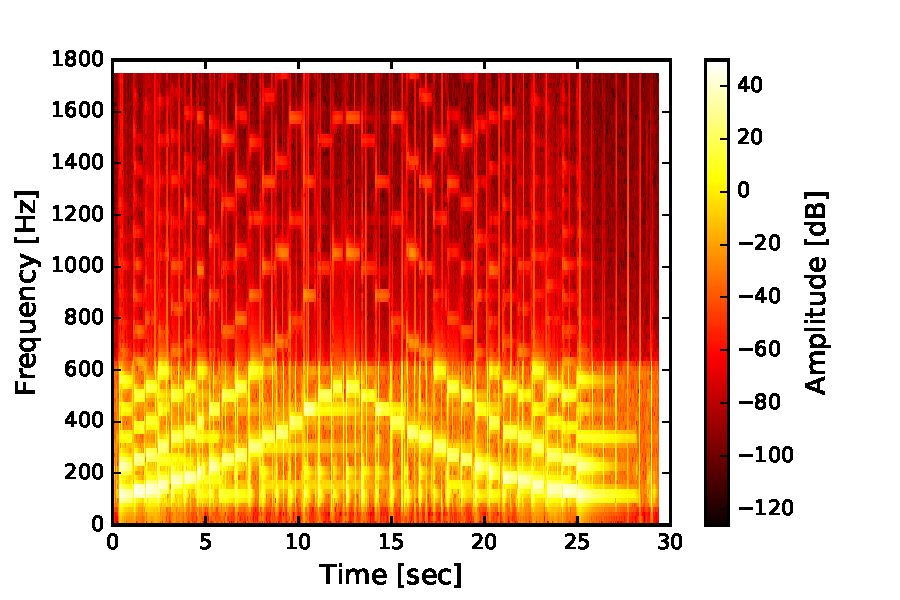
\includegraphics[width=\textwidth]{figures/validation/systemtest/final_spec.pdf}
\caption{Spectrogram}
\label{fig:final_spec1}
\end{subfigure}
\begin{subfigure}{0.49\textwidth}
\centering
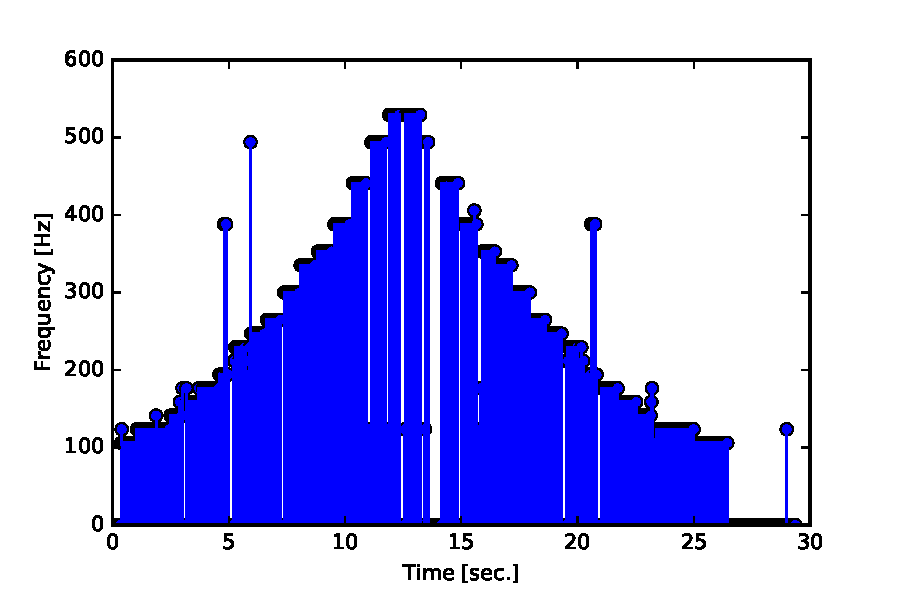
\includegraphics[width=\textwidth]{figures/validation/systemtest/final_peak.pdf}
\caption{Significant frequencies}
\label{fig:final_peak1}
\end{subfigure}
\label{fig:final_1}
\caption{Scale with clapping hands}
\end{figure} 
Figure \ref{fig:final_1} account for the system output of test 1. Bye this it is clear that the significant frequencies follows each scale. Though single incongruous frequencies appears, because of high\trine{low?} signal to noise ration within the passband at a certain time. From the result it is concluded that the scale is recognisable.  

\paragraph{Test 2} Melody "Lille Peter edderkop" by single tones with clapping hands.  
\begin{figure}[H]
\centering
\begin{subfigure}{0.49\textwidth}
\centering
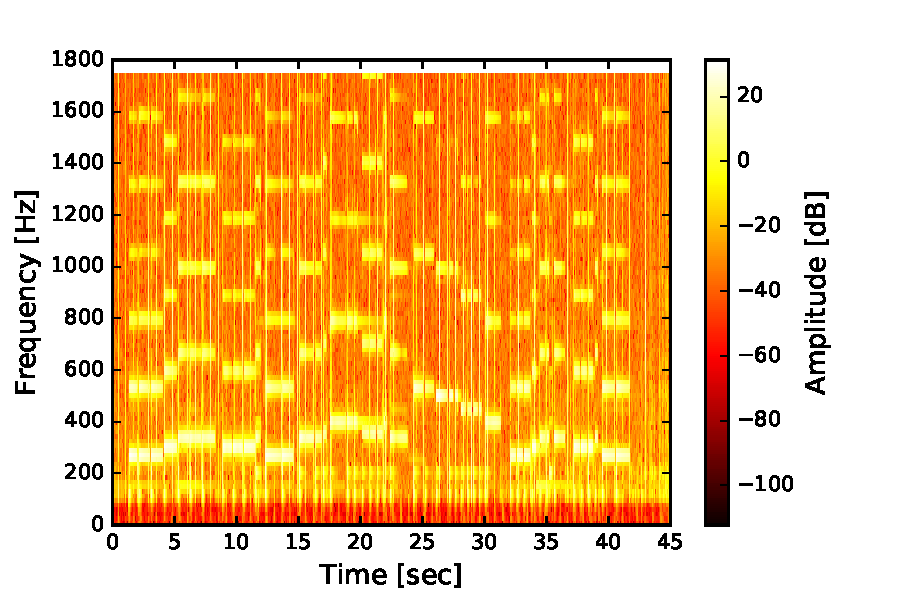
\includegraphics[width=\textwidth]{figures/validation/systemtest/final_spec3.pdf}
\caption{Spectrogram}
\label{fig:final_spec2}
\end{subfigure}
\begin{subfigure}{0.49\textwidth}
\centering
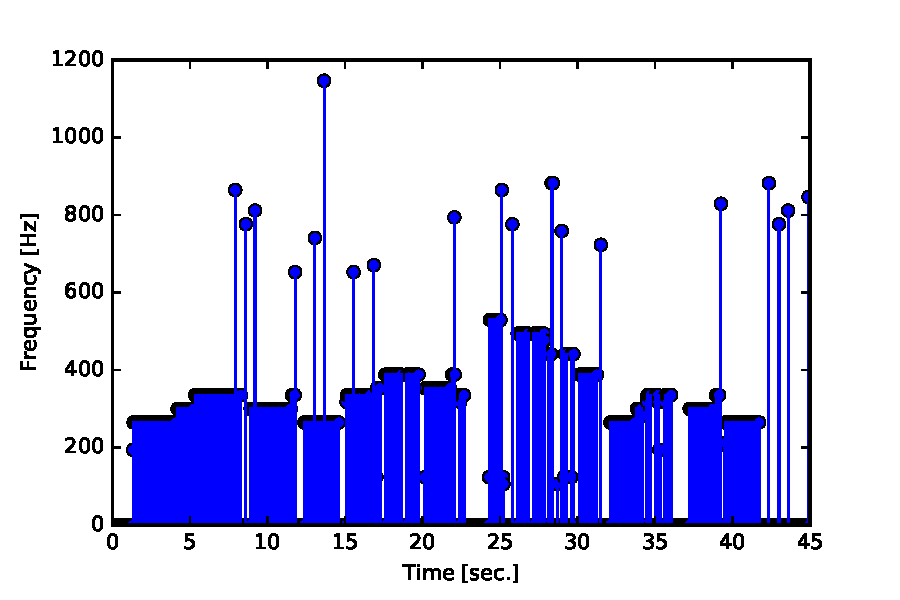
\includegraphics[width=\textwidth]{figures/validation/systemtest/final_peak3.pdf}
\caption{Significant frequencies}
\label{fig:final_peak3}
\end{subfigure}
\label{fig:final_3}
\caption{Melody "Lille Peter edderkop" by single tones with clapping hands.}
\end{figure}  

Figure \ref{fig:final_3} accounts for the output of test 2. It is seen compared to the result of the scale that the significant frequencies are not as clear caused by several incongruous detected frequencies though by ey         

\paragraph{Test 3} Low E cord with clapping hands
\begin{figure}[H]
\centering
\begin{subfigure}{0.49\textwidth}
\centering
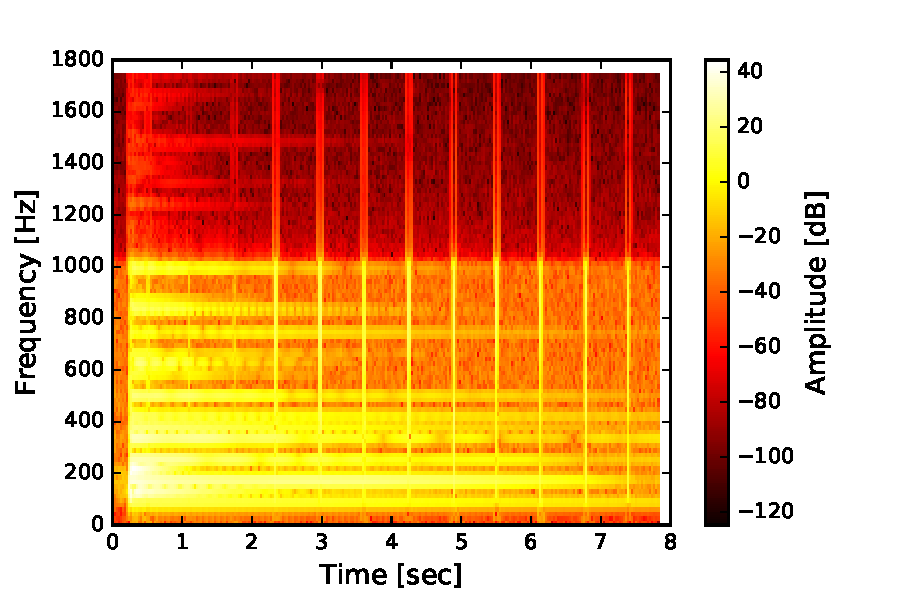
\includegraphics[width=\textwidth]{figures/validation/systemtest/final_spec2.pdf}
\caption{Spectrogram}
\label{fig:final_spec2}
\end{subfigure}
\begin{subfigure}{0.49\textwidth}
\centering
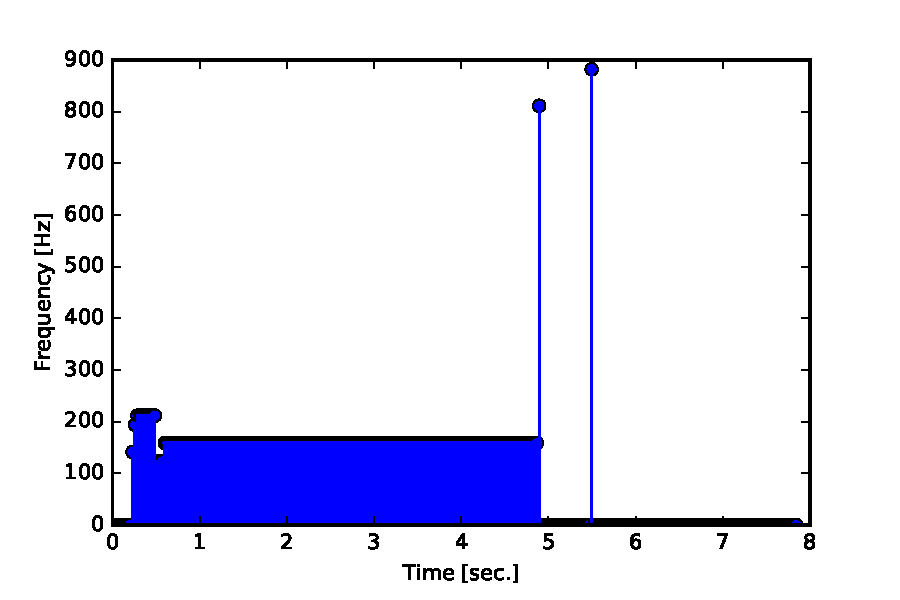
\includegraphics[width=\textwidth]{figures/validation/systemtest/final_peak2.pdf}
\caption{Significant frequencies}
\label{fig:final_peak2}
\end{subfigure}
\label{fig:final_2}
\caption{Low E cord with clapping hands}
\end{figure}  

Figure \ref{fig:final_3} accounts for the output of test 3. By the detected frequencies it is most likely to indicate that it is a single low E tone played rather than the low E cord played. This is expected because... \trine{some one?} 

\subsection{}